\documentclass{acm_proc_10ptArticle-sp}
\usepackage[T1]{fontenc}

\begin{document}

\title{Assignment 3 - Social Web}

\numberofauthors{3}
\author{
%
% The command \alignauthor (no curly braces needed) should
% precede each author name, affiliation/snail-mail address and
% e-mail address. Additionally, tag each line of
% affiliation/address with \affaddr, and tag the
%% e-mail address with \email.
\alignauthor Arthur-Ervin Avramiea\\
       \affaddr{2517642}\\
       \email{a.e.avramiea@student.vu.nl}
\alignauthor Mihnea Dobrescu-Balaur\\
	\affaddr{2549278}\\
	\email{mihnea@linux.com}
\alignauthor Zilvinas Kucinskas\\
	\affaddr{2547940}\\
        \email{zil.kucinskas@gmail.com}
}

\date{4 March 2014}
\maketitle

\section{Discuss an existing analysis}


During the recent years we have witnessed the explosion of the Web. It has become so popular that it is virtually omnipresent. Anywhere there is technology, you can find the Web. It is even on TVs. A big part of this evolution are the social networks - websites like Facebook, Twitter, MySpace etc. They allow people to easily communicate and share how they feel and what they are doing with their friends, and because of this, social websites (or their corresponding mobile apps) have become a part of most people's lives.

Now that the growth is starting to (relatively) cool down, it is good to analyze the numbers and get a good understanding of the trends that surround social media. The report "\textbf{Where in the World Are the Hottest Social Networking Countries?}"\footnote{http://www.emarketer.com/Article/Where-World-Hottest-Social-Networking-Countries/1008870} by \textit{emarketer} examines the spread of social network users across countries and looks at the overall growth of the number of users of the Social Web around the world.     

\subsection{About the data} 

The \textit{emarketer} report quantifies the use of social networking websites throughout the world, measuring their spread and predicting future numbers. 

There is data about Facebook users and Social Networking websites in general, on all devices, including mobile.

According to the report, the numbers are based on survey and traffic data from research firms and regulatory agencies. The predictions are based on trends observed by \textit{emarketer} and other country-specific socio-economic factors.

The demographics for this report are broad - people who access the internet from any kind of device. The data was clustered by country and region for one of the reports. Its geographic spread includes all the world, restricted to places that have Internet connectivity.

The report was released in February 2012 and covers the 2011-2014 period, meaning half of the data is predicted.


\subsection{Types of analyses}
The report contains three key points:

\begin{itemize}
\item the number of social users worldwide
\item the number of social users by region and country
\item the number of Facebook users worldwide
\end{itemize}

All of the data covers the 2011-2014 timeframe.

Considering that the report came out at the beginning of 2012, it means that the numbers for 2012, 2013 and 2014 are based on predictions formed by trend analysis.

In addition, the second point (number of social users by region and country) uses clustering to aggregate the numbers by country and region.

The three analyses don't look only at the absolute value of data, but also at the rate at which it is changing year by year. So, for example, the report predicts that Facebook's yearly increase of users will drop from 44\% in 2011 to 13.9\% in 2014.


\subsection{Limitations of the analyses}

The report is released by a research firm, and they favor their corporate subscribers. Because of this, the data that the report is based on is not released to the public. Moreover, there are no specifics mentioned about the size of the data, concrete sources etc. All that is mentioned is that the data is based on traffic data from "research firms" and other surveys. Because of this, the report can not be compared directly with others from the same sources, since those sources are unknown.

It is worth mentioning that the predictions it made were reasonably accurate - for example, the report predicted that Facebook will have 1.14 billion users in 2014, and the latest report says Facebook has 1.19 billion users.

While the report includes social users from Asia and makes claims about users in China, there are no mentions about other social networks. This is important, because Facebook was banned in China at the time of the report. It would have been useful for the report to include data about other social networks as well, especially since there are countries around the world (Brazil, Russia) where Facebook is not the most popular social network.


\section{Analysis of the geography of media influence}

Media, especially in the form of news sources, has a complex role in defining the way in which we perceive the side of the world that is near us, as well as the "other side" of the world. First of all, it can determine the priorities of the society, and influence our affinities. For example, as  \citeA{mccombs1972agenda} notes, the news media has a major influence on the topics around which a political campaign revolves. Second of all, news media can modulate our interest in specific national or international events \cite{wanta2004agenda}. Moreover, consumers judge the quality of the news by the extent to which the news meet their preconceptions and expectations\cite{gentzkow2005media}. 

In effect, the more homogenous the news sources to which a person is exposed, the less educated he/she may be about the topic. To resolve this issue, one can study various news sources when choosing which candidate to vote for in order to have a better impression of the advantages and disadvantages of each candidate choice. When one takes into account various international perspectives on external events, one may have a more complete and balanced image of the parties involved and the issues at stake. And even it involves an additional effort, reading news from sources that do not fit the individuals' preconceptions, or even contradict them, helps the individual understand the basis on which perspectives other than his own are grounded.

With the increased usage of the internet, users have access to sources other than the local or national news at the tip of their fingers. In this context, our research question is whether internet users take advantage of this opportunity, and access news originating from different countries, when informing themselves on an international topic. Although we are aware that different news agencies from the same country may reflect different perspectives on the same topic, we use the simplifying assumption that in sum, the news sources in a country reflect the country's stance on the topic.

To study how internet users access news sources we have chosen a subject that has generated a lot of controversy in the past days, the tensions in Crimea following the 18-23 Ukrainian revolution \footnote{http://en.wikipedia.org/wiki/2014\_Ukrainian\_revolution}. We have chosen this subject because it is likely to be treated differently by the media in different countries, depending on each country's stance on, and interests in, Crimea and the Ukrainian revolution.

\subsection{Data acquisition}

We have monitored the tweets which mention the keyword "crimea", using the Twitter Streaming API, over a time frame of 16 hours, between 12 and 13 March 2014, for a total of ~50.000 tweets on the subject. We needed to be able to associate each tweet to the country in which the user is located. Only a few of the tweets are tagged with an exact location. Where that field was not available, we used the user's location, when that was specified. An issue is that the user location field is not very exact - the user can specify any string of characters to describe his location: "Portland, OR, United States" (which points to an actual location) or "Around you" (as ambiguous as it can get). We used the Google Places text search API to extract the location from this text (if it was possible). Although this approach is not the most accurate, we think it suffices for the purposes of this work. We were able to extract the country for 20.786 tweets, which we used afterwards in our analysis.

For each tweet we were interested by the following information: the tweet's text(to be used for sentiment analysis), the urls to which the tweet refers (to analyse the news sources) and the user's location. 

From Twitter, for each tweet, we received a lot of unneeded information: 

\begin{verbatim}
{
    \\info about tweet
    "text": "Vice News has some...,
    "id": ...,
    "favorite_count": 0,
    "entities": {
        \\info about other entities
        "urls": [
            {
               \\info about urls
               "expanded_url": "...",
            }
        ]
    },
    "user": {
        "location":"Olympia",
        \\information about the user
    },
    ...
    "place": null
}
\end{verbatim}

For each place, we got from the Google Places API the following information: 
\begin{verbatim}
{
    "Batam, Indonesia": {
        "geo_location": {
            "lat": 1.0456264,
            "lng": 104.0304535
        },
        "address": "Batam, Riau Islands, 
                         Indonesia"
    }
}
\end{verbatim}

From this, we have extracted the country from the last part of the address.

In order to assess the country for a news source, we have used the country top level domain list\footnote{http://en.wikipedia.org/wiki/List\_of\_Internet\_top-level\_domains}. The rest of the websites, with non-national domain names (.com, .org, .info etc) were classified by hand (only the most popular ones). 

Integrating this data for each tweet results in the following data representation, that fits the purposes of our analysis, and in which we have the location of the tweeter and the location of each url referred in the tweet:

\begin{verbatim}
 {
    "text": "Russia's 25,000-troop...",
    "urls": [
        {
            "url": "http://rt.com/news/r...",
            "country_code": "RU"
        }
    ],
    "country_code": "SK"
}
\end{verbatim}

\subsection{Analysis of the data}

As you can see in Fig. \ref{fig:toptweets} the countries from which the highest numbers of tweets originate are: USA(8022), United Kingdom (1698), Ukraine(1089), Spain(1057) and Canada(896). USA is present in the top due to its large number of tweeter users and of news agencies. Ukraine is the hot spot, so no wonder that we find it in the top. However, the other 3 countries share something in common with Ukraine - they all have debates regarding the separation of a region from the country, as it is the case now for Crimea in Ukraine. Independence processes are undergoing for Catalonia in Spain\footnote{http://www.catalannewsagency.com/politics/item/the-new-york-times-editorial-catalan-secession-claims-are-legitimate-not-like-crimea-s}, Quebec in Canada, and Scotland in UK\footnote{http://en.wikipedia.org/wiki/Scottish\_independence\_ referendum,\_2014}.

Our main question concerns which news sources do internet users access - local(national) news or international news. For this, we have computed the local news access index (LNAI) - which for each country, is computed as the percentage of local(national) websites mentioned in the tweets of users from that country, in all the websites mentioned by the same users. In Fig. \ref{fig:mediacoverage} you can see a map of the local news access index. The highest values for LNAI (eliminating countries with less than 10 tweets) were found in Spain (0.44), Italy(0.39), Russia (0.38). This shows the preponderence of local media in these countries. However, this does not completely describe the influence of the local media in those countries, as users may have other reasons for not accessing external sources - such us the fact that they do not speak a foreign language. 

Interestingly, LNAI for Ukraine is small(0.23), and although users mostly access news sources from Ukraine and Russia, not a few users are watching the news from USA (Fig. \ref{fig:sources_ukraine}) .

The LNAI for USA is also small, with only 17\% of the references made to local news. The rest of it reflects the ethnic diversity in the USA, as well as the broad coverage of external news in US media (Fig. \ref{fig:sources_usa}) . 

On the other side of the spectrum, as we have already mentioned, we have countries like Russia, with a preponderence of local media on the subject, seconded by USA and then Ukraine \ref{fig:sources_russia}.

We have also performed a sentiment analysis of the tweets, using the sentiment140 API\footnote{http://www.sentiment140.com/}. The results for each country can be found on the map \ref{fig:sentimentmap} . The sentiment score was computed by summing the tweets with negative polarity (multiplied by -1) with the tweets with positive polarity (multiplied by 1), and dividing this by the total number of tweets originating in each country. The result was then rescaled from 0 to 10, where 0 means negative polarity, 5 neutral, and 10 positive. We expected to find heterogeneity in the emotional content that surrounds the subjects. However, the results are quite homogenous - for most of the countries, the overall score was neutral, and the rest is noise, due to the small number of tweets. 

\subsection{Conclusions}

A first issue that we encountered was that of identifying the country to which a news source belongs. Some urls which did not have a national top level domain were left out because we did not have the time to manually classify them. For future studies it would be useful to identify lists of news agencies and their details, and automatize the process of country identification, whenever possible. 

Overall, our intention was to see whether internet users access news from multiple sources. Although in many countries we could see a heterogenous set of data sources, this heterogenous data set is more likely to represent different subsets of the population which take their information from different sources, rather than one individual with a broad coverage of the media. In that case, this would unravel the heterogeneity of the population with regard to the news sources that are used. A further study should take this analysis to a deeper, individual level, and assess the extent to which users access a heterogenous set of news sources. 

We need to also take into account that the average Twitter user may not be representative for the rest of the internet users population. For example - Twitter users may be more exposed to disparate news sources, and hence be more likely to access them. As such, the observations and conclusions should not be generalized to the rest of the population. 

With regard to the sentiment analysis, as you could see, the results were quite homogenous. There are several possible reasons for this finding. First of all, the query may have been too general ("crime") - a more specific query like "putin crimea" could have reflected a more polarized view. Second, the percentage of tweets with emotion was quite small (at most 10\% of the tweets), and for countries with a small number of tweets, it may not have been enough to properly describe the overall sentiment. Moreover, our metric divides the sum of positive and negative tweets to the total number of tweets. Given the small percentage of polarized tweets, this results in an inherently neutral score. We would need to find a better metric to properly reflect the overall sentiment. 

All in all, we consider that our study gives an answer to the research question. The user of the internet has access to multiple news sources and takes advantage of this opportunity. However, deeper analyses may prove useful in describing the intricacies of the news browsing behavior. Moreover, analyses that take into account the globalization of news media can uncover the influence that a certain event has on other places and peoples. An example is the report in the news of the possible separation of Crimea, which spawns debates in countries like Canada, UK, Spain, that are discussing the possible separation of certain regions. 

% The following two commands are all you need in the
% initial runs of your .tex file to
% produce the bibliography for the citations in your paper.
\bibliographystyle{abbrv}
\bibliography{assignment3}

\newpage

%Appendix A
\onecolumn
\section{Appendix}
\begin{figure}[H]
	\centering
	\includegraphics[width=0.9\linewidth]{crimea_tweets.png}
	\caption{Top tweets about crimea}
	\label{fig:toptweets}
\end{figure}

\begin{figure}[H]
	\centering
	\includegraphics[width=0.9\linewidth]{media_coverage.png}
	\caption{Media coverage - for each country, the percentage of local media mentions, in the total number of tweet url mentions}
	\label{fig:mediacoverage}
\end{figure}

\begin{figure}[H]
	\centering
	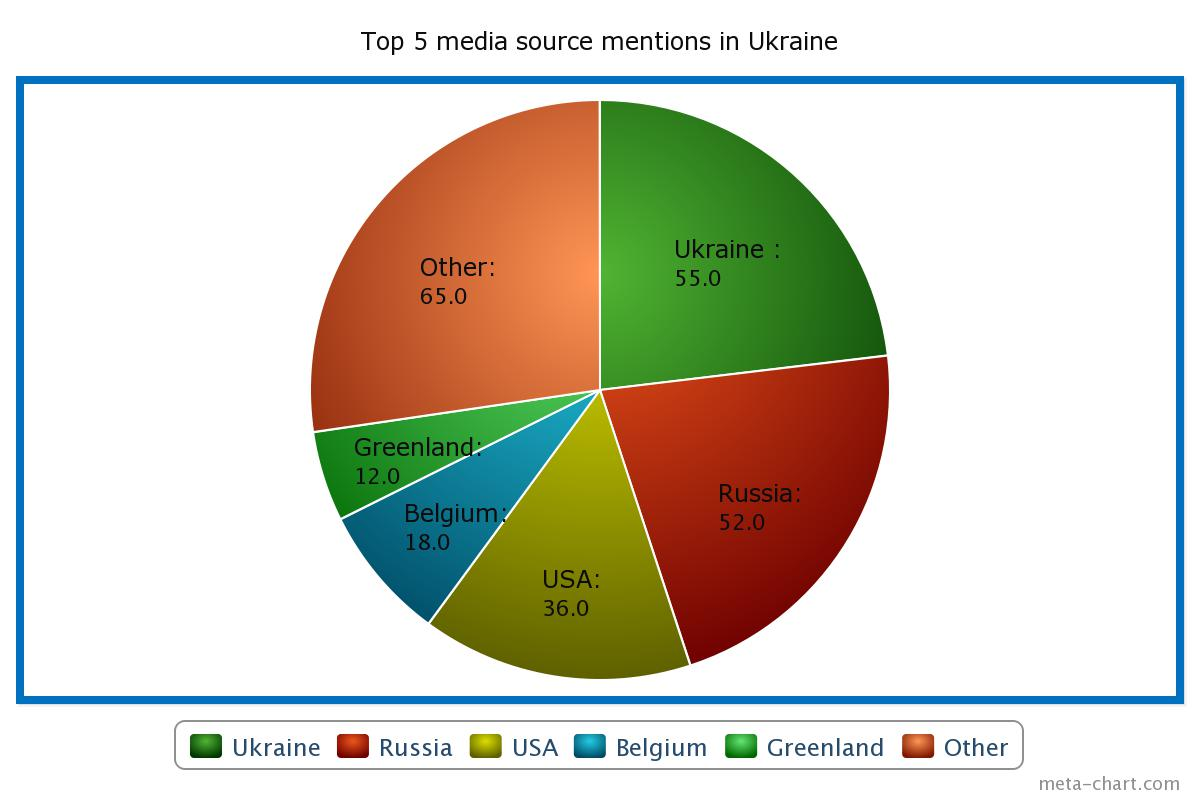
\includegraphics[width=0.9\linewidth]{topMentionsInUkraine.jpeg}
	\caption{News sources mentioned in tweets originating from Ukraine}
	\label{fig:sources_ukraine}
\end{figure}

\begin{figure}[H]
	\centering
	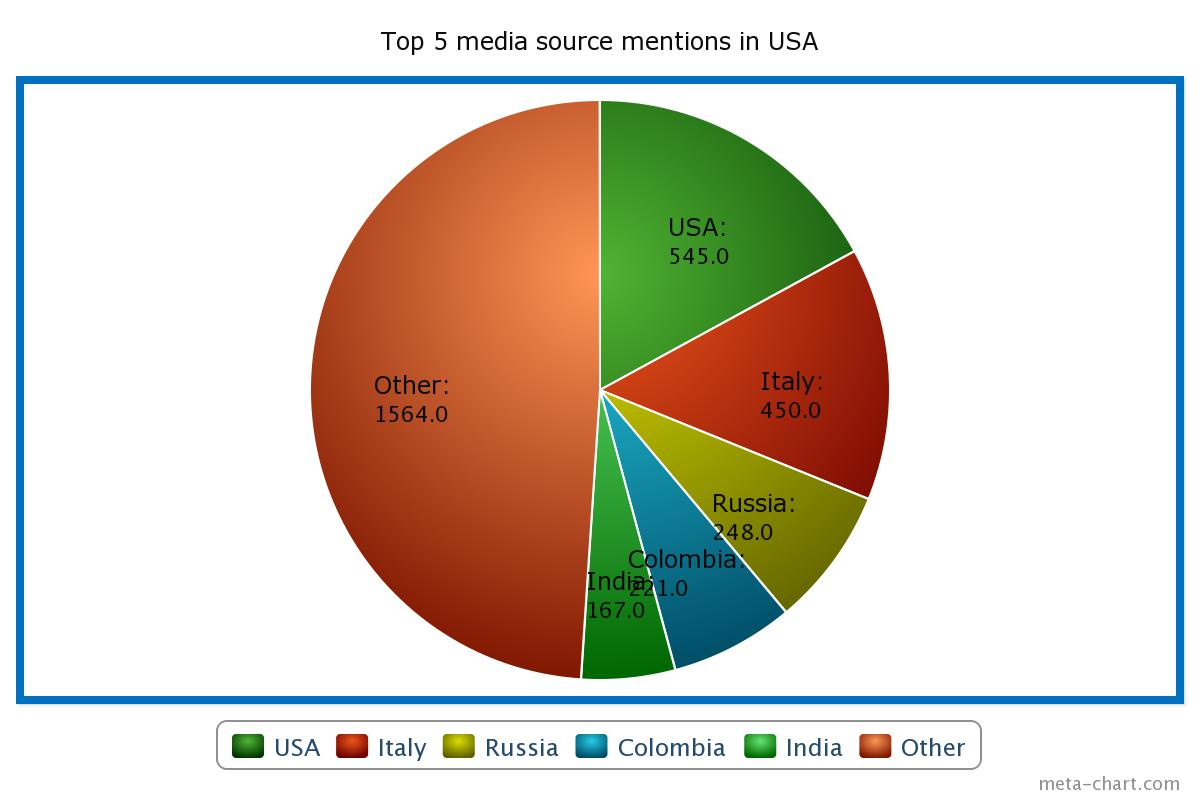
\includegraphics[width=0.9\linewidth]{topMentionsInUSA.jpeg}
	\caption{News sources mentioned in tweets originating from USA}
	\label{fig:sources_usa}
\end{figure}

\begin{figure}[H]
	\centering
	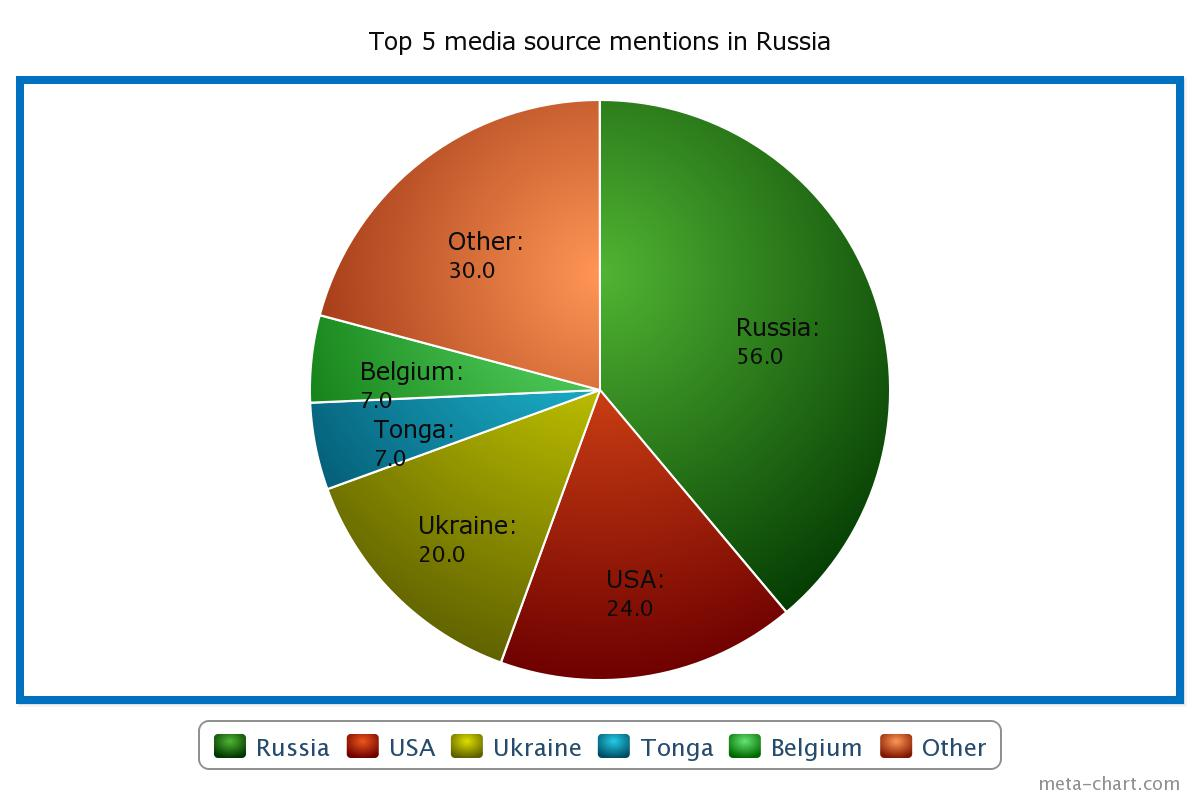
\includegraphics[width=0.9\linewidth]{topMentionsInRussia.jpeg}
	\caption{News sources mentioned in tweets originating from Russia}
	\label{fig:sources_russia}
\end{figure}

\begin{figure}[H]
	\centering
	\includegraphics[width=0.9\linewidth]{crimea_sentiment.png}
	\caption{Sentiment analysis}
	\label{fig:sentimentmap}
\end{figure}


\end{document}